





\documentclass[12pt,letterpaper,notitlepage]{article}
\usepackage{graphicx}
\usepackage{float}
\usepackage{epsfig,epsf}
\usepackage{epstopdf}
\usepackage{curves}
\usepackage{hyperref}
% The following packages are important as they allow to write certain mathematical expressions.
\usepackage{amsmath}
\usepackage{amssymb}
\usepackage{color}
% To write a code in a LaTeX document you need:
\usepackage{listings}
\definecolor{dkgreen}{rgb}{0,0.6,0}
\definecolor{dkblue}{rgb}{0,0.0,0.6}
\definecolor{dkred}{rgb}{0.9,0.0,0.1}
%% Own definitions:
\newcommand{\BEq}{\begin{eqnarray}}
\newcommand{\EEq}{\end{eqnarray}}
\newcommand{\BEqn}{\begin{eqnarray*}}
\newcommand{\EEqn}{\end{eqnarray*}}
\newcommand{\BM}{\begin{subequations}}
\newcommand{\EM}{\end{subequations}}
\newcommand{\BEqM}{\begin{subequations}\begin{eqnarray}}
\newcommand{\EEqM}{\end{eqnarray}\end{subequations}}
\newcommand{\Bitem}{\begin{itemize}}
\newcommand{\Eitem}{\end{itemize}}
\newcommand{\Ben}{\begin{enumerate}}
\newcommand{\Een}{\end{enumerate}}
%% Greek letters:
\renewcommand{\a}{\alpha}
\renewcommand{\b}{\beta}
\newcommand{\D}{\Delta}
%% Colors:
\newcommand{\TB}[1]{\textcolor{blue}{#1}}
\newcommand{\TR}[1]{\textcolor{red}{#1}}
\newcommand{\bm}[1]{\mbox{\boldmath $#1$}}
\newcommand{\non}{\nonumber\\}
%% Some simplified expressions:
\def\eps{\varepsilon}
\def\r{\right}
\def\l{\left}
\def\p{\partial}
\def\d{\delta}
\newcommand{\ta}{\mbox{$\theta$}}
\newcommand{\ve}{\mbox{${\cal E}$}}
\newcommand{\etab}{\bar{\eta}}
\newcommand{\sg}{\tilde{\sigma}}
\newcommand{\tap}{\mbox{$\theta'$}}
\newcommand{\tta}{\mbox{$\tilde{\theta}$}}
\newcommand{\ttap}{\mbox{$\tilde{\theta}'$}}
\newcommand{\taz}{\mbox{$\theta_0$}}
\newcommand{\phip}{\mbox{$\phi'$}}
\newcommand{\tphi}{\mbox{$\tilde{\phi}$}}
\newcommand{\tphip}{\mbox{$\tilde{\phi}'$}}
\newcommand{\ty}{\mbox{$\tilde{y}$}}
\newcommand{\gb}{\mbox{$\bar{\gamma}$}}
\newcommand{\gone}{\mbox{$\gamma_1$}}
\newcommand{\gtwo}{\mbox{$\gamma_2$}}
\newcommand{\phiz}{\mbox{$\phi_0$}}
\newcommand{\Nf}{\mbox{$N_f$}}
\newcommand{\Nv}{\mbox{$N_v$}}
\newcommand{\qt}{\mbox{$\tilde{q}$}}
\newcommand{\qa}{\mbox{$q_\alpha$}}
\newcommand{\tqa}{\mbox{$\tilde{q}_\alpha$}}
\newcommand{\dqa}{\mbox{$\delta q_\alpha$}}
\newcommand{\pqa}{\mbox{$\partial_{u} q_\alpha$}}
\newcommand{\pqta}{\mbox{$\partial_{u} \tilde{q}_\alpha$}}
\newcommand{\pdqa}{\mbox{$\partial_{u}\delta q_\alpha$}}
\newcommand{\sn}{\mbox{${\rm sn}$}}
\newcommand{\cn}{\mbox{${\rm cn}$}}
\newcommand{\dn}{\mbox{${\rm dn}$}}
\newcommand{\cd}{\mbox{${\rm cd}$}}
%%% Creation, destruction operators:
\newcommand{\cks}{\mbox{$c_{{\bf k},\sigma}$}}
\newcommand{\cksd}{\mbox{$c_{{\bf k},\sigma}^\dagger$}}
\newcommand{\cku}{\mbox{$c_{{\bf k},\uparrow}$}}
\newcommand{\ckd}{\mbox{$c_{-{\bf k},\downarrow}$}}
\newcommand{\ckud}{\mbox{$c_{{\bf k},\uparrow}^\dagger$}}
\newcommand{\ckdd}{\mbox{$c_{-{\bf k},\downarrow}^\dagger$}}

\begin{document}

\lstset{language=Fortran,tabsize=4,numbers=left,numberstyle=\tiny,basicstyle=\ttfamily\small\color{dkblue},stringstyle=\ttfamily\color{blue},keywordstyle=\rmfamily\color{dkred}\bfseries\emph,backgroundcolor=\color{white},commentstyle=\color{dkgreen}}




\title{%
	Chaotic Behavior of Driven and Damped Harmonic Oscillator  \\
\large Computional Physics - Phys 562}
\author{Benjamin Deutsch  \\
Department of Physics\\
California State University Long Beach}
\date{\today }

  
\maketitle



\begin{abstract}
Here we will utilize the Fortran 95 Programming environment to execute a program to plot a driven, and damped harmonic oscillator (pendulum). Within the program we will use a Runge Kutta 4 step iterative subroutine. To demonstrate chaotic behavior we will plot  $\omega$ against the driving force $g$, the emergent map is seen to produce a number of bifurcations. Multiple runs were then executed in order to generate a denser graph with clearer chaotic regions.        
\end{abstract}

\section{Introduction}

With regards to modern physics many new fields attract a great level interest, however in the older topic of mechanics there exists regions of still considerable research possibilities, one such is in the area of chaotic systems. Chaos, as motion is defined to be contained in a system who's initial conditions are very specific and motion is deterministic, there exist unpredictability in the long term behavior of the system. This idea extends to many every day occurrences such as the cooling of hot coffee, the motion of traffic and even weather forecasting. We explore this idea simplifying it to the behavior of only a driven, damped harmonic oscillator, a tool regularly explored in physics. Left alone, a simple harmonic oscillator will enjoy a predicable pendular motion, we then here introduce damped and driving terms to bring different sensitivity to the initial conditions. With the changing of the damping force and resulting affected angular frequency $\omega$ at different points in time, the picture arises of data points  located in both dense and sparse regions. Through iterating in time the points tend to attract in certain dense branch areas, describing selected areas of angular frequency. More interestingly we can see broad areas fill with a multitude of points, analysis in this regime, we understand this a chaotic region by the inability to select the next outcome. These terms in this case can and do localize to a remaining branch and the bifurcation process begins again.  The use of the main routine alleviates the extremely laborious nature of single calculation, the computer gives us the ability to investigate not only the obviously chaotic behavior but also the effective change of it given certain initial conditions, such as the bifurcation problem described in the results. Some new tools are used in the coding such as the RK 4 step subroutine command which will organize and make the code more user friendly.           


\section{The Math and Theory}

For the assignment we are asked to use the dimensionless driven damped oscillator see here,

	\begin{equation}
	{\frac{d^2\theta}{dx^2}+\frac{1}{q}\frac{d\theta}{dt}+sin\theta=g\cos(W_D t)}	
	\end{equation}
\\
For this q is the damping term, g the forcing amplitude and the W the angular driving frequency. 
To place make this easier to visualize and place into the programming environment, we must separate the terms; 
\\
	\begin{equation}
	{\frac{dW}{dt}=-\frac{1}{q}W-sin\theta+g\cos\phi}
	\end{equation}	
\\
	\begin{equation}
	{\frac{d\theta}{dt}=W}
	\end{equation}
\\
	\begin{equation}
	{\frac{d\phi}{dt}=W_D}	
	\end{equation}
\\
Here we have complementary set of first order equations, which can be readily entered into the RK 4 step subroutine for call into the main routinue.  

\section{The code}

To begin the Fortran code we must use a module that declares the variables of the use internal to the called subroutine so that the variables are understood in both files. Once this is done we can declare the usual variables, integers, and arrays, some needed in the exterior subroutine. Next we have included  in the header the declaration of constants as well as simply equations needed to define further variables i.e. step size. 

The loop included in the main program, is uniquely interesting for a number of reasons, one of which is that it only looks at a very small region of values living within .9 and 1.6, this is guided by the prescribed text on the assignment. The loop also contains a determined step on which to plot. Second is the nested do loop which incorporates the \textbf{while} command, this is needed so that a determined condition can be established "while" another process is being used. Here the conditions are implement so that unusably high and low values are corrected. 

As this code needs many mapped points, we can limit the time variable so to only plot the last remaining and normally the more informative of the points. This done by using the last 90\% of the time steps, as to not get lost in the sea of early non effected points. Finally after this has been all been taken care of we for each of these do loops the result (g, Y(1)) is written to a exterior \textbf{.fort} file extension by a \textbf{write} command to graphed externally. 
\newpage
\section{Results and Conclusion}	
	\begin{figure}[H]
		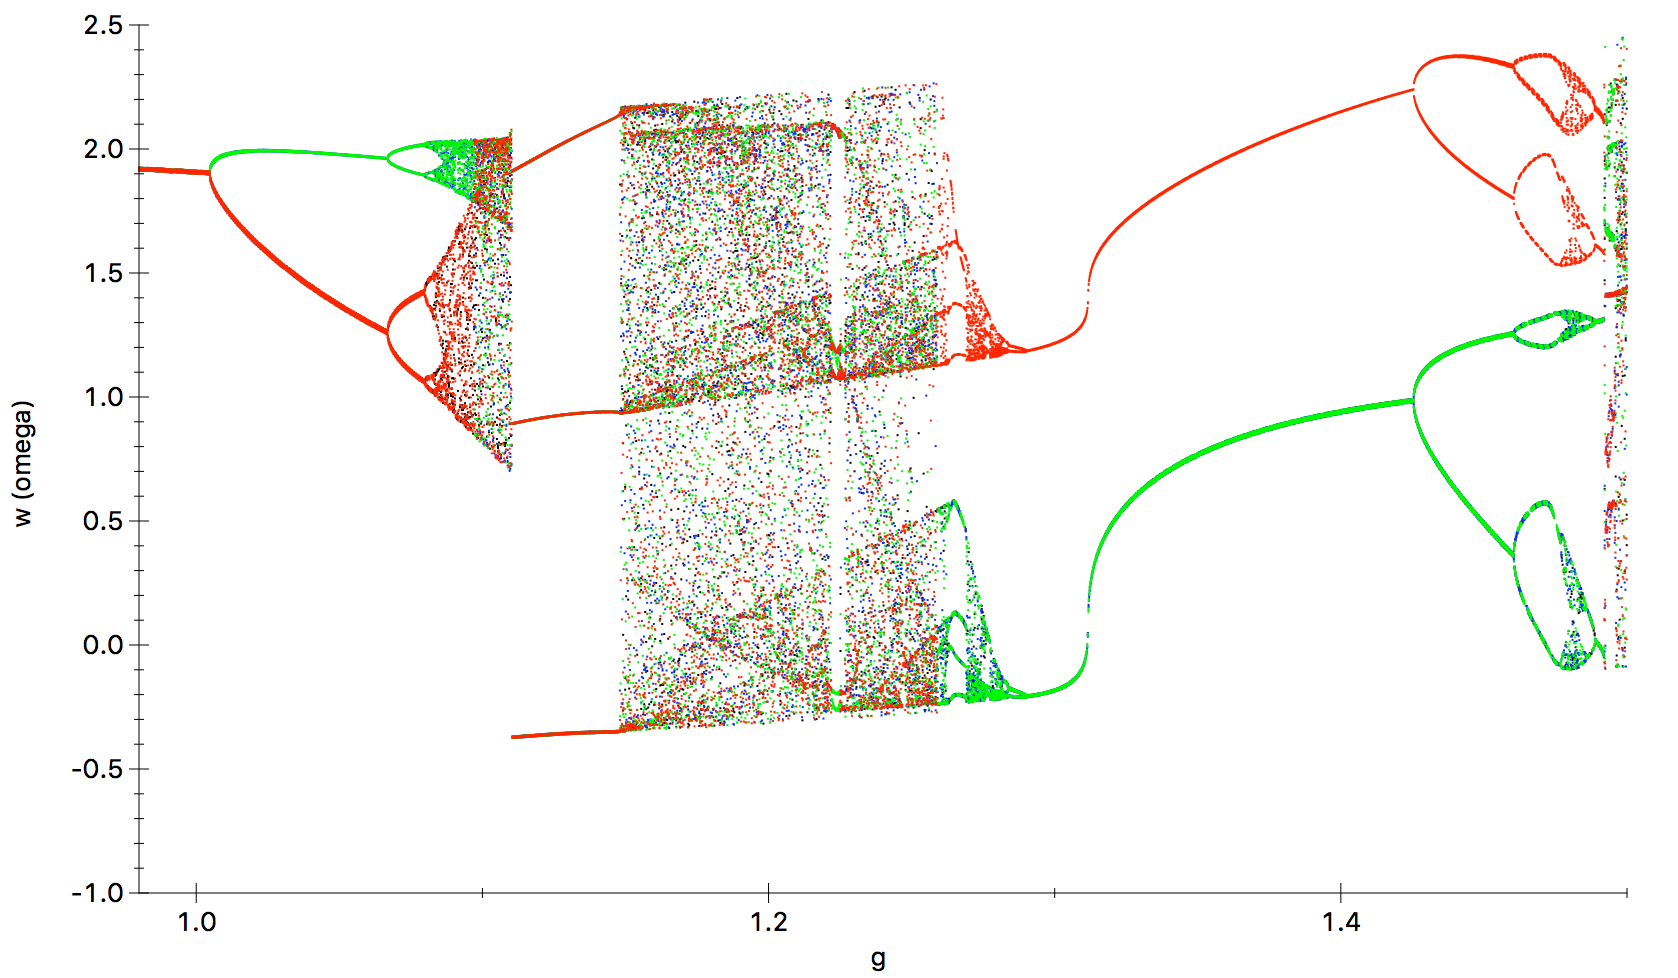
\includegraphics[width=1.\textwidth]{bif.png}
		\caption{Chaotic behavior of damped harmonic oscillator, between $\omega$= -1.0, 2.5 ; g=1.0, 1.9}
	\end{figure}  
	\begin{figure}[H]
		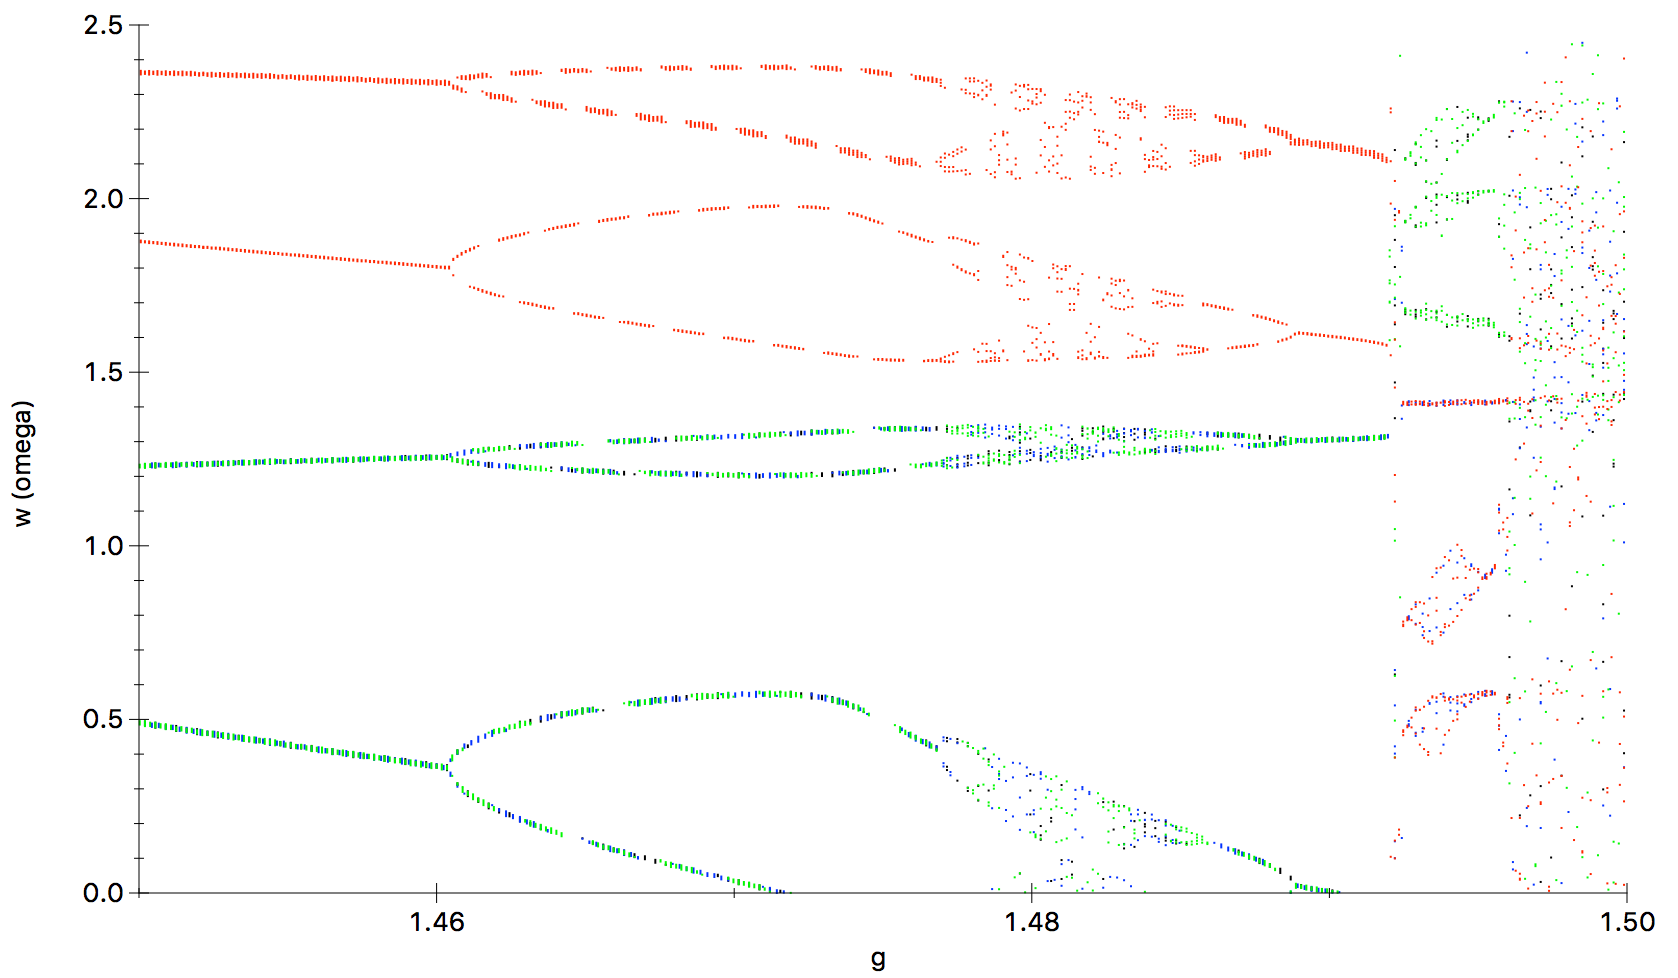
\includegraphics[width=1.\textwidth]{bif2.png}
		\caption{Detailed look at unique bifurcation to chaotic behavior} 
	\end{figure}    
To illustrate the chaos of the system multiple runs above been preformed, each with greater iteration ranging from 2000 to 5000 points (Blue, 2000; Green, 3000; Orange, 4000; Red, 5000). These plots have been superimposed atop each other to form Figure 1. A more detailed look at one area shown in Figure 2, gives us a better interpretation of these dynamic systems, while selecting an intial condition, step size, we have already influenced the outcome and bifurcations of the plot. The chaotic behavior of the system can be seen in large strokes such as areas between g values of 1.15 and 1.25. In conclusion the resulting graph does resemble the literature example and the project was seen as a success. In which we can understand the motions of chaotic systems and how they manifest in time.   
\newpage
\begin{thebibliography}{}
 \bibitem{1}
	Z.~Papp and A.~Bill, {\it Computational Physics Lecture Notes}, California State University Long Beach.

\end{thebibliography}




\end{document}








